\section{Lecture 14 - 10/07/2022}

\subsection{Generalized Cauchy's Theorem}

Last class, recall we discussed the Generalized Residue Theorem, whose proof relied on Theorem~\ref{thm::zero_path_thm}. 
 Theorem~\ref{thm::zero_path_thm} above is sometimes called the \textbf{Generalized Cauchy's Theorem}, not to be confused with the \textbf{Generalized Residue Theorem} that we proved last lecture.

\begin{theorem}
    Let $\gamma$ be a generalized closed path (ie. it is a union of finitely many closed paths) in $\Omega$, such that for all $z \notin \Omega$,
    \[w(\gamma, z) = 0\]
    Then, we have that for all $f \in Hol(\Omega)$,
    \[\int_\gamma f(z) dz = 0\]
\end{theorem}

Before proving this, we will first state a lemma:

\begin{lemma}
    Let $K$ be a compact subset of open $\Omega$ (ie. $K \subset \Omega$), then there exists some bounded open set $G$ with $\partial G \in PC^1$ such that:
    \begin{itemize}
        \item $cl(G) \subset \Omega$
        \item $dist(K, G^c) \geq \delta > 0$
    \end{itemize}
\end{lemma}

\begin{proof}
    Since $K$ is compact and $\Omega^c$ is closed, we know that $dist(K, \Omega^c)$ must be positive (or else they would intersect). So let's pick some $\delta$ such that $dist(K, \Omega^c) \geq 4 \delta > 0$.\\\\
    Now consider a $\delta$-grid of $\Omega$ (split $\Omega$ into squares of side length $\delta$), and consider
    \[G \coloneqq int(\bigcup_{\text{$Q$ is a square on the $\delta$-grid,}\ dist(K, Q) \leq \delta} Q)\]
    Note, that we might create a $G$ where it does have a self-intersection on the boundary, which would not make it $PC^1$, in this case, we would add a little square on the corner to ``nudge" the boundary away:
    \[\fbox{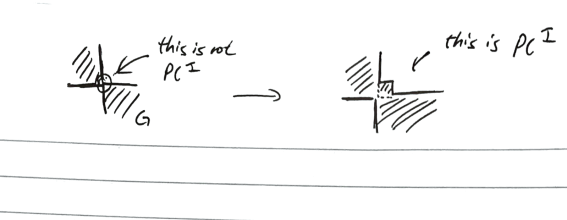
\includegraphics[width=.5\textwidth]{Figures/pc1.png}}\]
    Then we can check that
    \[dist(K, G^c) = dist(K, \partial G) \geq \delta\]
    If this is not true, then our $G$ would have to be surrounded by other cubes whose distance to $Q$ is less than $\delta$, and hence we are not looking at the boundary of $G$.
\end{proof}


\begin{proof}[Proof of Theorem~\ref{thm::zero_path_thm}]
    Recall that $f \in Hol(f)$, and consider
    \begin{align*}
        \int_\gamma f(z) dz &= \int_\gamma \frac{1}{2\pi i} \int_{\partial G} \frac{f(\xi)}{\xi - z} d\xi dz \tag*{Since f is holomorphic, use Cauchy's Integral Formula}\\
        &= \int_{\partial G} \frac{-f(\xi)}{2\pi i} \int_\gamma \frac{1}{z - \xi} dz d\xi \tag*{Fubini's Theorem}
    \end{align*}
    Now for any $\xi \in \Omega^c$, we claim that
    \[\int_\gamma \frac{1}{z - \xi} dz = 0\]
    Since $G \subset \Omega$, we have that $\Omega^c \subset G^c$. Thus, any connected component of $\Omega^c$ is contained in some connected component of $G^c$.\\\\
    If a bounded connected component $C$ of $G^c$ does not intersect with $\Omega^c$, we just add it to $G$ (take $G'$ = $G \cup C$ to be the new $G$). So we can without loss assume that any bounded component of $G^c$ intersect with $\Omega^c$.\\\\
    Thus, for all $\xi$ in such bounded component of $G^c$, 
    \[\int \frac{1}{z - \xi} dz = 0\]
    Indeed, consider the diagram:
    \[\fbox{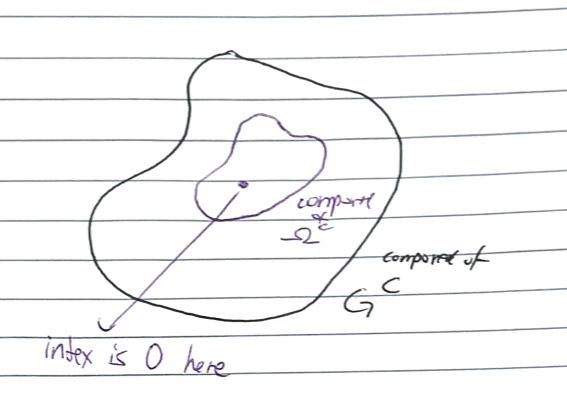
\includegraphics[width=.5\textwidth]{Figures/bounded_zero.png}}\]
    Recall that by assumption, the index of any point in $\Omega^c$ is $0$. Since the winding number is an analytic (thus continuous) function, this means that the index of every point on this one bounded component of $G^c$ is identically zero.\\\\
    Now, on unbounded connected components of $G^c$, we can't just add this to $G$ since we still want $G$ to be bounded. But we note that $W(\gamma, \xi) = 0$. This is because as $|\xi| \to \infty$, we can eventually find some $\xi$ such that the loop $\gamma$ does not enclose it. The fact that the entire component has index $0$ follows from the fact that the winding number is a continuous function. \\\\
    Thus, we have that
    \[\int_\gamma f(z) dz = \int_{\partial G} \frac{-f(\xi)}{2\pi i}  \cdot 0 d\xi  = 0\]
\end{proof}

\begin{remark}
    On the complex plane $\Cbb$, we can add a point at infinity as the one-point compactification of $\Cbb$, which we denote as $\hat{\Cbb}$. This is called the \textbf{Riemann Sphere}.\\\\
    Then on $\hat{\Cbb}$, $\Omega$ is a simply connected domains if and only if $\hat{\Cbb} \setminus \Omega$ is connected. The proof in the book is rather tedious and uses many details, but there's a standard topological proof of this using the Riemann Mapping Theorem, which we will discuss later.
\end{remark}

\begin{corollary}
    Let $\Omega \subsetneq \Cbb$ be a bounded domain and $\Cbb \setminus \Omega$ is connected, then for any $z_0 \in \Cbb \setminus \Omega$, there exists a branch of $\log(z - z_0)$ in $\Omega$.
\end{corollary}

\begin{proof}
    Fix some $w_0 \in \Omega$ and take $a_0$ as one of the values of $\log (w_0 - z_0)$ (this is defined up to $2\pi i$, but we just choose one). Now we define the branch $\log z - z_0$ as
    \[\log(z - z_0) = a_0 + \int_{w_0}^z \frac{d\xi}{\xi - z_0} \]
    Note that our integral does not depend on the choice of pathes, as shown by the Generalized Cauchy's Theorem, so our branch is well-defined.
\end{proof}

\subsection{Jump Theorem for Cauchy Integrals}

Let $\gamma$ be a $C^1$-curve and suppose $f$ be a $C^1$ compact-supported function on $\gamma$ (denote this as $f \in C^1_c(\gamma)$, note this need not be analytic). We want $f$ to be compactly supported to avoid any convergence issue.

There's a slight abuse of notation going on here, by $f \in C^1(\gamma)$, we actually mean that for $\gamma: [a, b] \to \Cbb$, $f \circ \gamma$ is $C^1$.

Define the function
\[F(z) \coloneqq \frac{1}{2\pi i} \int_\gamma \frac{f(\xi)}{\xi - z} d\xi\]

We note that $F \in Hol(\gamma^c)$, now take some point $z_0 \in \gamma$, and consider
\[F_{\pm}(z_0) \coloneqq \lim_{z \to z_0} F(z)\]
, where ``$+$" is from inside and ``$-$" is from outside.\\\\

Naively, we claim we could just exchange the limit and the integral, then
\[F_{\pm}(z_0) = \frac{1}{2\pi i} \int_{\gamma} \frac{f(\xi)}{\xi - z_0} d\xi\]

However, in general the integral is not integrable around $z_0$, so we next hope that we could converge it to some principal value:
\[F_{\pm}(z_0) = \frac{1}{2\pi i} p.v. \int_{\gamma} \frac{f(\xi)}{\xi - z_0} d\xi\]
, where we say that
\[p.v. \int_\gamma ... = \lim_{\delta \to 0} \int_{\gamma \setminus D_{z_0, \gamma}} ...\]

This, however, is also problematic! Indeed, consider the following counter-example where $\gamma$ is a circle and $f(z) = 1$ is the constant $1$ function:
    \[\fbox{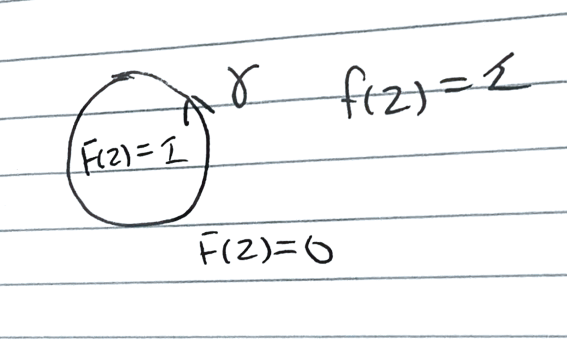
\includegraphics[width=.5\textwidth]{Figures/cauchy_jump.png}}\]
, but $F(z)$ is the winding number and is hence $1$ inside and $0$ outside. So the limit does not even converge.

The next best thing we get, is fortunately true. This is sometimes also called the \textbf{Jump Theorem}:

\begin{theorem}[Plemelji-Sokhotsky formula]
    \[F_{\pm}(z_0) = \frac{1}{2\pi i} p.v. \int_\gamma \frac{f(\xi)}{\xi - z_0} d\xi \pm \frac{1}{2} f(z_0)\]
\end{theorem}

\begin{remark}
    Note that the theorem is actually also true for just curves (need not be closed). In this case, by inside and outside we mean the orientation given by the \textbf{left leg rule}.
\end{remark}

Before we prove the theorem, we first make an observation:
\begin{observation}\mattie{Why??}
    We note that the theorem is actually a local theorem. If $f \in C^1(\gamma)$ and $f \equiv 0$ in a small neighborhood of $z_0$, then everything is trivial as
    \[F_{\pm}(z_0) = \frac{1}{2\pi i} \int \frac{f(\xi)}{\xi - z_0} d\xi\]
    Therefore, we can without loss just assume $f \in C^1(D_{z_0, \delta_0})$.
\end{observation}

\begin{proof}[Proof of Jump Theorem]
    \begin{align*}
        \int_\gamma \frac{f(\xi)}{\xi - z_0} d\xi &= \int_\gamma \frac{f(\xi) - f(z)}{\xi - z} d\xi + \int_\gamma \frac{f(z)}{\xi - z} d\xi
    \end{align*}
    Note that as we take $z \to z_0$ on the left integral, we can apply the Dominated Convergence Theorem as $|\nabla f| \leq M$ in $D_{z_0, \delta_0}$ is bounded on compact set, and everything is compactly supported
    \begin{align*}
        \lim_{z \to z_0}  \int_\gamma \frac{f(\xi) - f(z)}{\xi - z} d\xi &= \int_\gamma \lim_{z \to z_0} \frac{f(\xi) - f(z)}{\xi - z} d\xi \tag*{Dominated Convergence Theorem}\\
        &= \int_\gamma \frac{f(\xi) - f(z_0)}{\xi - z_0} d\xi\\
        &= p.v. \int \frac{f(\xi)}{\xi - z_0} d\xi - p.v. \int_\gamma \frac{f(z_0)}{\xi - z_0} d\xi \tag*{Existence of Principal Values left as Exercise}
    \end{align*}
    For the right integral, we will evaluate
    \begin{align*}
        \lim_{z \to z_0} \int_\gamma \frac{f(z)}{\xi - z} d\xi
    \end{align*}
    We will finish the proof in the next lecture.
\end{proof}